\begin{figure}[h!tb]
    \centering
    \captionsetup{type=plot}
    \caption{\label{plot:matrix}Effective bandwidth by $b$ size}
    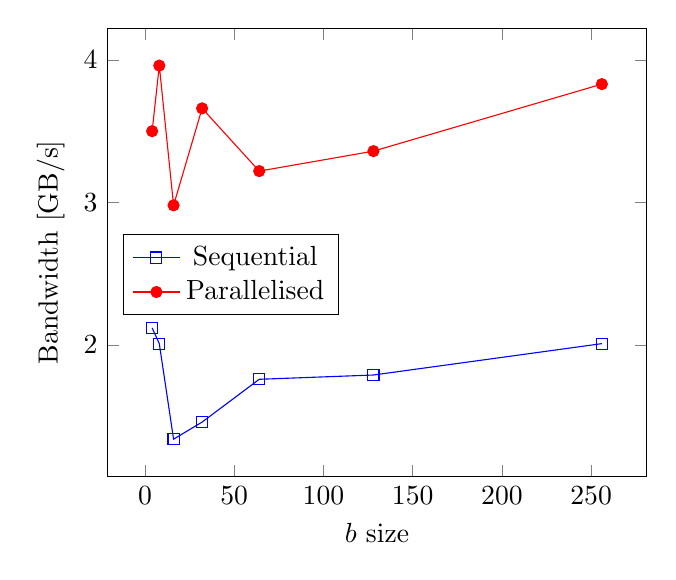
\begin{tikzpicture}
        \begin{axis}[
            title={},
            xlabel={$b$ size},
            ylabel={Bandwidth [GB/s]},
            legend style={at={(0.03,0.45)},anchor=west}
        ]
            \addplot[
                color=blue,
                mark=square,
                ]
                coordinates {
                    (4,2.12)
                    (8,2.01)
                    (16,1.34)
                    (32,1.46)
                    (64,1.76)
                    (128,1.79)
                    (256,2.01)
                };
            
            \addplot[
                color=red,
                mark=*,
                ]
                coordinates {
                    (4,3.50)
                    (8,3.96)
                    (16,2.98)
                    (32,3.66)
                    (64,3.22)
                    (128,3.36)
                    (256,3.83)
                };
            \legend{Sequential, Parallelised}
        \end{axis}
    \end{tikzpicture}
\end{figure}